\section{Background, \mtl Problem and Our Approach}
\label{sec:problem}
\label{sec:prob-def}

In this section, we describe the background of the shared spectrum systems,
formulate the \mtl problem, then describe our methodology. 

\para{Shared Spectrum System.} In a shared spectrum paradigm, the
spectrum is shared among licensed users (primary users, PUs) and
unlicensed users (secondary users, SUs) in such a way that the
transmission from secondaries does not interfere with that of the
primaries (or secondaries from a higher-tier, in case of a multi-tier
shared spectrum system). In some shared spectrum systems,
the location and transmit power of the primary users may be
unavailable, as is the case with military or navy radars in the CBRS band.
%%%%%
Such sharing of spectrum is generally orchestrated by a centralized
entity called {\em spectrum manager}, such as a spectrum
database in TV white
space~\cite{sas-paper} or a central spectrum access system in
the CBRS 3.5GHz shared band~\cite{milind2015dyspan}. The spectrum
manager allocates spectrum to requesting secondaries (i.e., permission
to transmit up to a certain transmit power at their location) appropriately
so as to avoid interference with primaries.
%%%%%%%%%%%%
Users who transmit without explicit permission are referred to as 
unauthorized users or {\em intruders}; the \mtl problem is to essentially
localize such intruders. 

\para{\mtl Problem.}  Consider a geographic
area with a shared spectrum. Without loss of generality, we assume a
single wireless frequency\footnote{To avoid confusion with image channels, we use {\em wireless frequency} instead of the perhaps more appropriate {\em wireless channel} term.} throughout this paper\footnote{Multiple wireless frequencies can be handled independently. 
Note that if we assume the wireless propagation characteristics to be similar for different frequencies, then we do not need to train different models for each of them. Our localization techniques would still work
for scenarios wherein the intruders may change their transmit frequencies dynamically.}.
For localization of intruders, we assume
available crowdsourced sensors that can observe received signals in the wireless frequency of interest, and compute (total) received signal strength (RSS).
RSS can be measured using low-cost sensors and has been shown to achieve good accuracy for single-transmitter localization~\cite{infocom00-radar}.
In the related work Section~\ref{sec:wowmom-related}, we will discuss signal metrics other than RSS, such as AoA, ToA, etc.~At any instant, there may be a set of intruders
present in the area with each intruder at a certain location transmitting
with a certain power which may be different for different intruders.
%%%%%%%%%%%%%%%%%%%%%%%%%%%

The \mtl problem is to determine the set of intruders with their
locations at each instant of time, based on the set of sensor
observations at that instant. 
%%%%%
For the main 
\mtl problem, we assume that there are no primary or authorized users, and thus, assume that the
sensor readings represent aggregate received power from the transmitters we
wish to localize.
However, in Section \ref{sec:authorized}, we investigate the more general \mtl problem where the background primary and/or secondary users may also be present.

\begin{figure*}
    \centering
    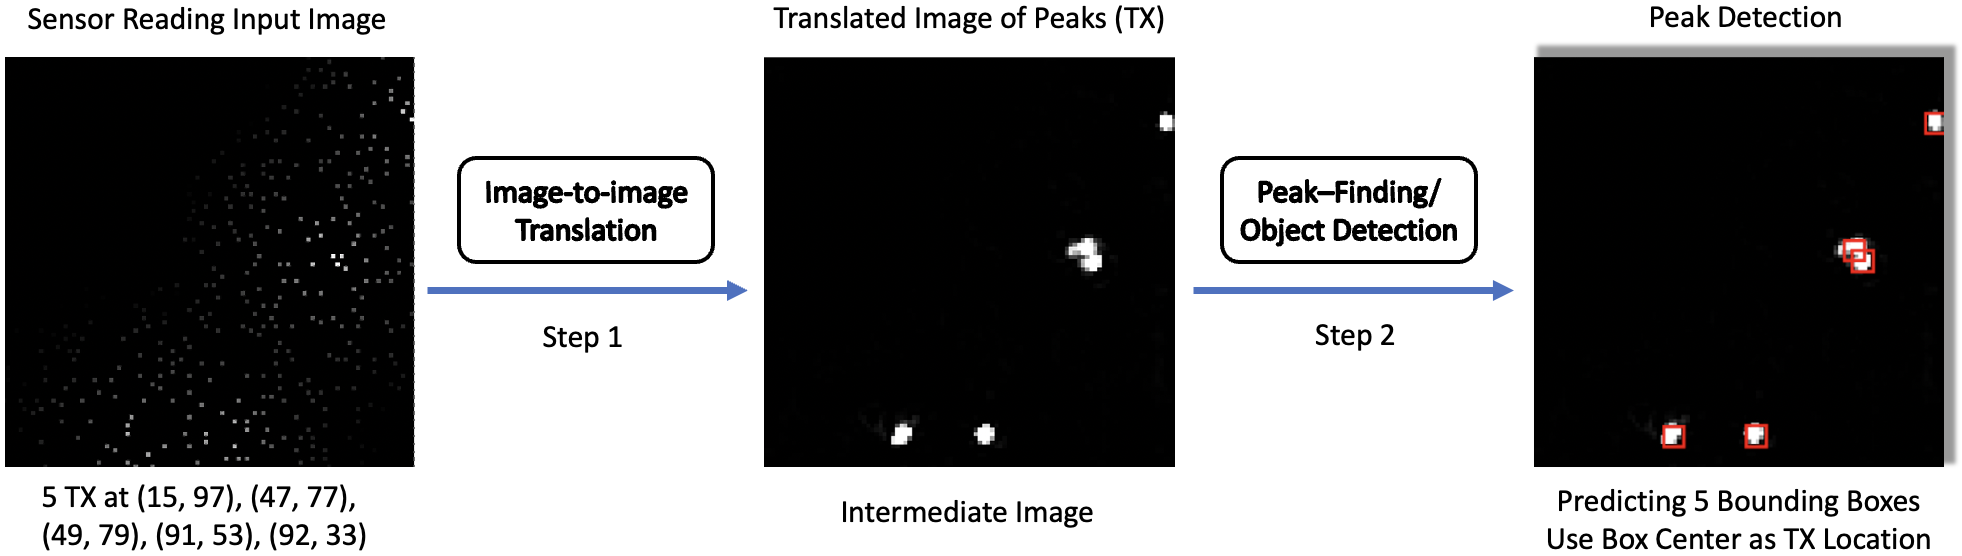
\includegraphics[width=\textwidth]{chapters/wowmom-pmc/figures/two-step-idea.png}
    \caption{The overall two-step CNN architecture of the \our model. The first step is the \imgimg, 
    whose higher idea is to translate the input image of sensor readings to the image of peaks where each peak implies a transmitter. 
    The \imgimg architecture is illustrated in Fig.~\ref{fig:part1}. The second step is \yolocust, a customized version of YOLOv3, 
    to perform object/peak detection in the output image of the first step. This step returns the precise location coordinates of TX. 
    The \yolocust architecture is illustrated in Fig.~\ref{fig:yolo}. A zoom-in of the peak detection result of the second step is in Fig.~\ref{fig:peaks}.}
    \label{fig:overall}
\end{figure*}

\para{\bf Our Approach.}
In our context, each sensor communicates its observation to a centralized spectrum 
manager which then runs localization algorithms to localize any potential (multiple) transmitters. 
%%%%%%%%%%%%%%%%%%%%%
We design and implement a novel two-step localization algorithm named \our, as illustrated in Fig.~\ref{fig:overall}, based on CNN models. 
The first step (Section \ref{sec:translate}) is a four-layer image-to-image translation CNN model that is trained
to translate an input image representing sensor readings to an image of 
transmitters' locations distributions. Each distribution of a transmitter can be visualized as a mountain with a peak, so we name this model \imgimg.
The second step (Section \ref{sec:detect}), called \yolocust, is a customized object-detection method built upon YOLOv3\cite{yolov3} which localizes the objects/peaks in the translated image.
%%%%%%%%%%%%%%%%%%
The high-level motivation behind our two-step design is to frame the overall \mtl
problem in terms of well-studied learning problem(s). 
The two steps facilitate efficient learning of the models by supplying an intermediate image with the training samples. 
%With this design, we fix the drawback in~\cite{icccn20-deeptxfinder} that needs to train a large number of models and it is way more accurate. We elaborate the step 1 in Section \ref{sec:translate} and step 2 in Section \ref{sec:detect}.
%}
